\chapter{Introducción}
\thispagestyle{empty}


\section{Marco temático}
\subsection{Esculturas cinéticas}
\subsubsection{Definición}
Las esculturas cinéticas (kinetic sculpture en inglés) son estructuras tridimensionales en donde el movimiento es una parte fundamental del conjunto. Para lograr el efecto de movimiento en el espacio estos sistemas se construyen con partes móviles que pueden cambiar de posición ya sea naturalmente por acción del viento, como se ve en la figura \ref{fig:1.1}, o de manera forzada. \\
% https://www.youtube.com/watch?v=D2HF-1xjpP8

\begin{figure}[!ht]
	\centering
	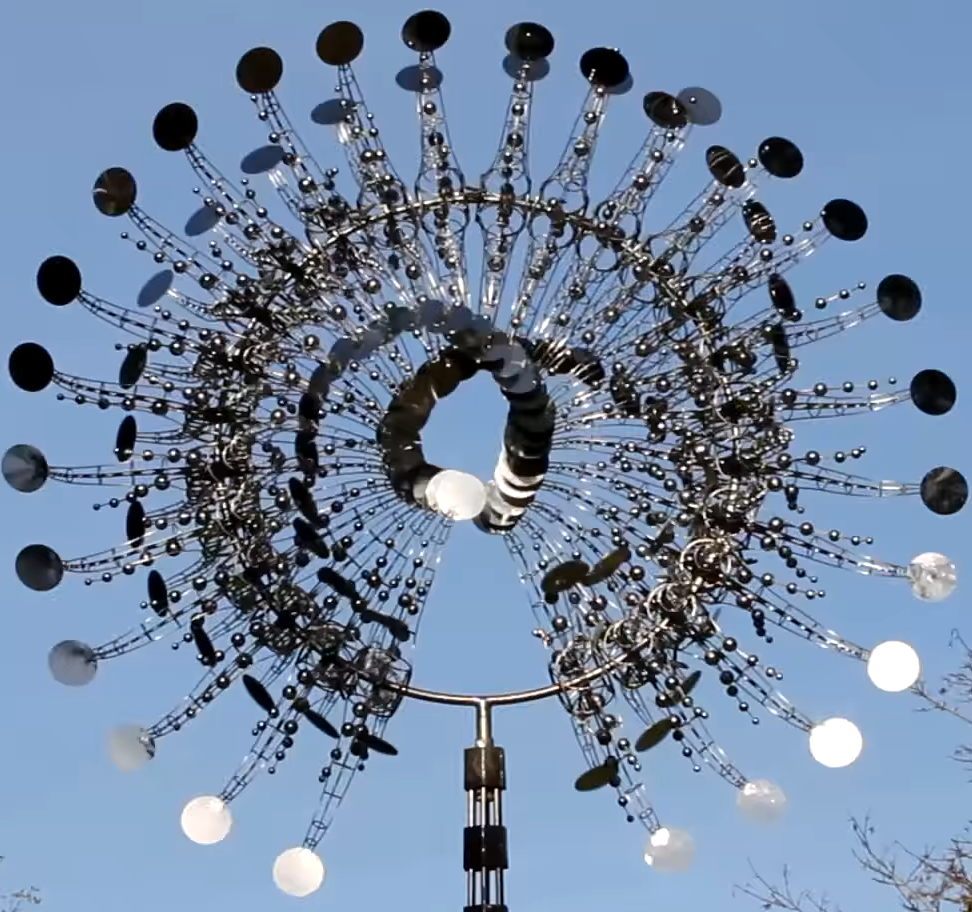
\includegraphics[width=10cm,scale=1]{resources/1_1-kinSculp.png}
	\caption{ Ejemplo de escultura cinética movida por aire, por Anthony Howe. Fuente:  \href{https://www.youtube.com/watch?v=N-1LpikCSR4}{LINK al video} }
	\label{fig:\thefigure}
\end{figure}

\newpage
\subsubsection{Aplicaciones y estado actual del arte}
Al ser obras que caen dentro del campo artístico suelen presentarse en museos y utilizarse para fines decorativos ya sea en parques o eventos. Sin embargo, el nivel de ingeniería y diseño que algunas de ellas requieren las tornan un interesante desafío intelectual y creativo.\\


Las aplicaciones puntuales de estructuras cinéticas a las que se hará foco en este informe, debido a la naturaleza del proyecto final, son aquellas en donde el efecto espacial se logra a través del movimiento en el eje vertical de objetos esféricos mediante motores. \\

Un ejemplo de aplicación de estas características se puede ver en la figura \ref{fig:1.2}. Allí se muestra una escultura presentada en el Museo de BMW, en Munich, Alemania, en donde 714 esféras metálicas son coordinadas para formas figuras como olas, gotas, y hasta la silueta de un auto \\
\begin{figure}[!ht]
	\centering
	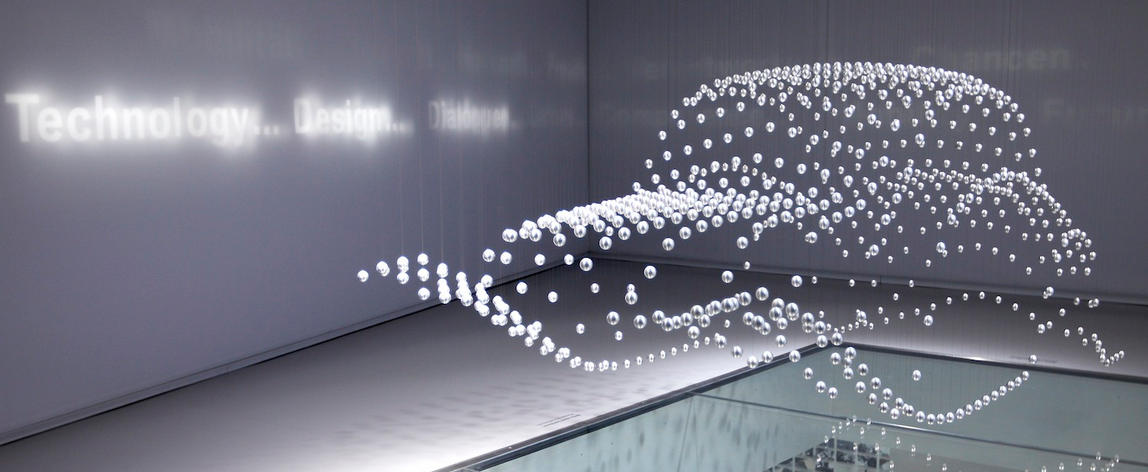
\includegraphics[width=15cm,scale=1]{resources/1_2-kinSculp.png}
	\caption{ Escultura cinética en el museo BMW. Fuente: \href{https://www.youtube.com/watch?v=HVhVClFMg6Y}{LINK al video} }
	\label{fig:\thefigure}
\end{figure}

Otro ejemplo de aplicación se puede ver en la figura \ref{fig:1.3}, en una obra presentada por la empresa Build Up en un centro comercial en Fukuoka, Japón. Allí se instalaron 1000 luminarias esféricas RGB dispuestas en una matriz de 25x40 para generar figuras tridimensionales como planos y gausseanas, entre otras. En este caso los efectos espaciales se logran coordinando el movimiento de cada esfera independientemente, cada una manejada por un equipo motorizado.
\begin{figure}[!ht]
	\centering
	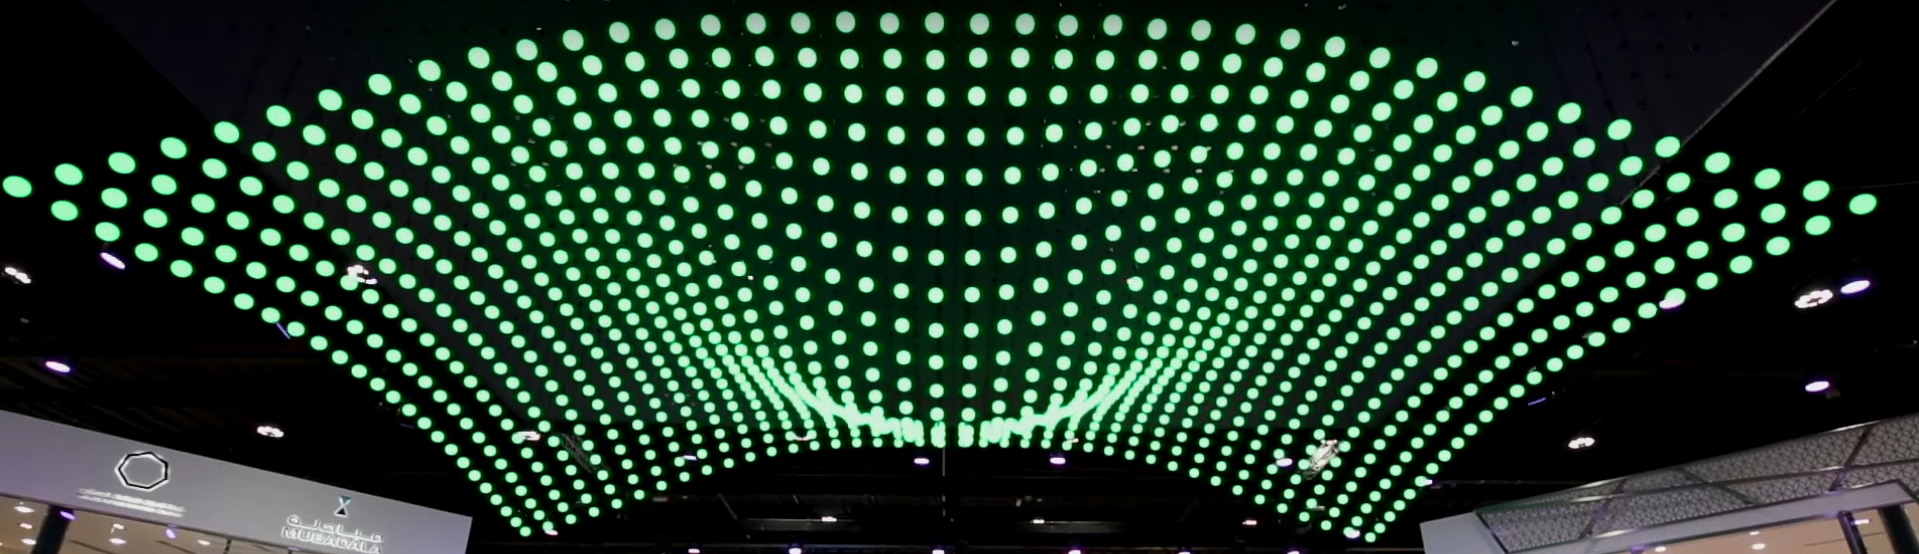
\includegraphics[width=15cm,scale=1]{resources/1_3-kinSculp.png}
	\caption{ Escultura cinética por parte de Build Up. Fuente: \href{https://www.youtube.com/watch?v=ICixCazf6-k}{LINK al video} }
	\label{fig:\thefigure}
\end{figure}

%\newpage


\subsection{Sistemas de iluminación}
\subsubsection{Equipos de luces}
En cualquier espectáculo o evento la iluminación es una parte vital del show, y a medida que estos fueron evolucionando también lo hicieron los equipos de luces. Partiendo de aparatos fijos en donde solo se podía variar la intensidad de luz, se pueden conseguir hoy en día dispositivos complejos con decenas de parámetros controlables.\\
Un notable ejemplo es el \href{http://preworks.at/index.php/en/products/led-automated-luminairies/shapeshifter}{Shapeshifter}, figura \ref{fig:1.4}, que cuenta con 7 módulos leds que pueden ser manejados independientemente.

\begin{figure}[!ht]
	\centering
	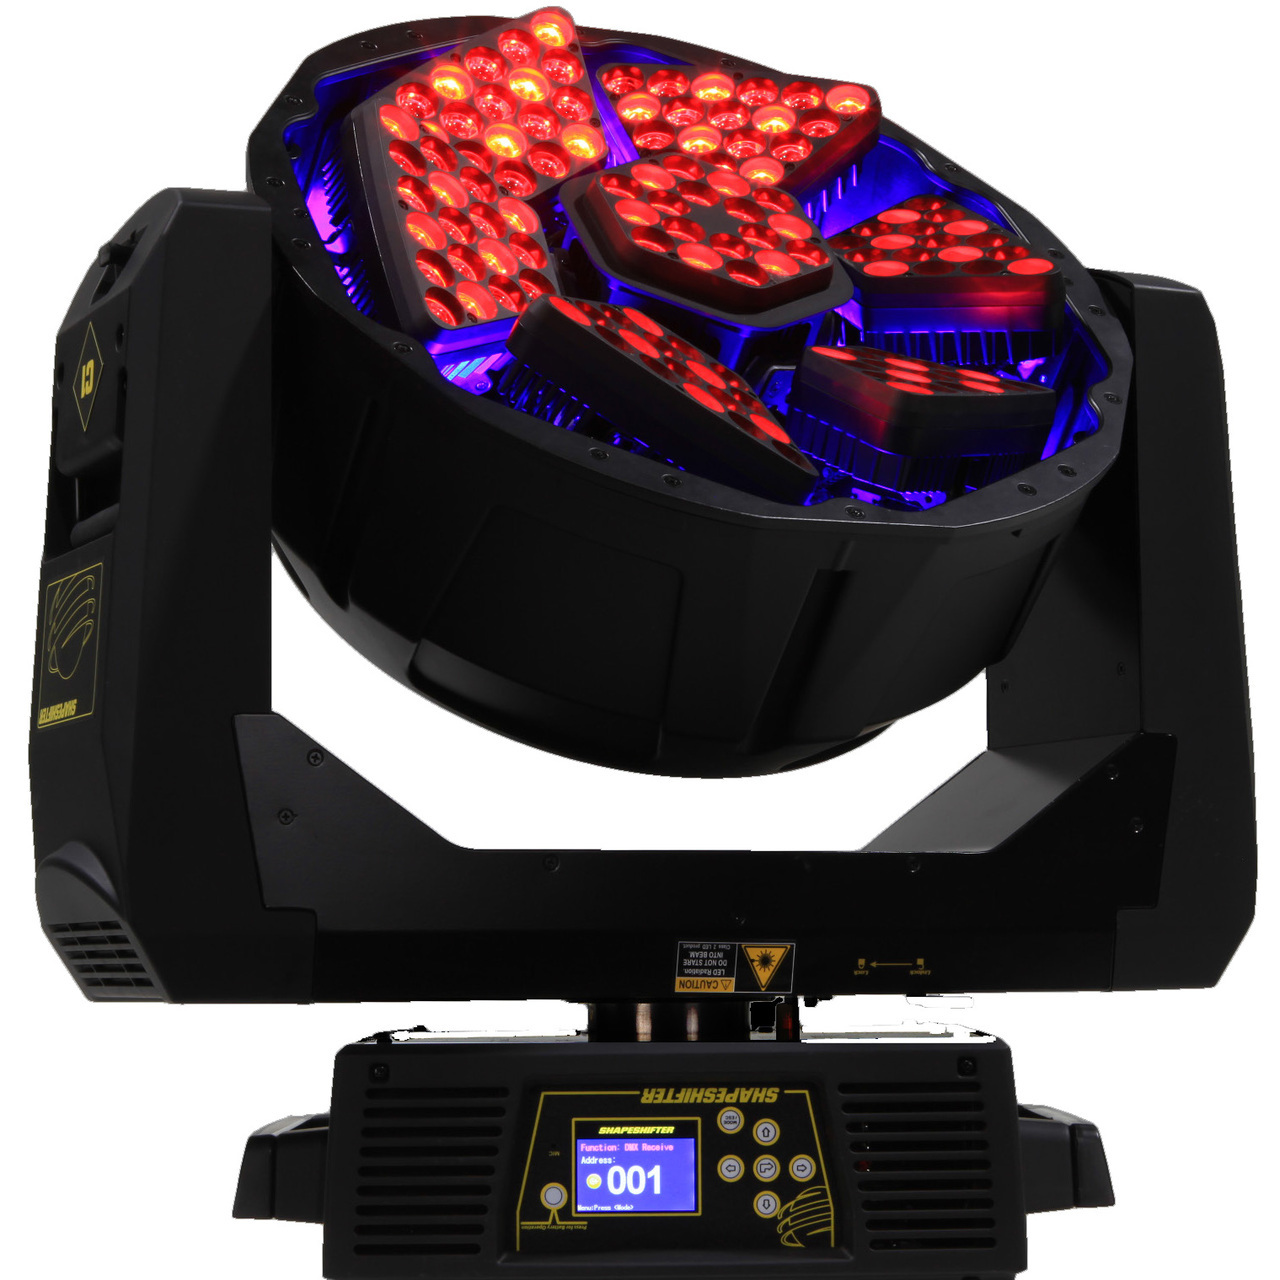
\includegraphics[width=7cm,scale=1]{resources/1_4-shapeshifter.jpg}
	\caption{Shapeshifter, de High End Systems. Fuente: \href{https://www.youtube.com/watch?v=LIIE3zZscYY}{LINK al video} }
	\label{fig:\thefigure}
\end{figure}

En el caso del sistema visto en la figura \ref{fig:1.3}, los parámetros controlables de los equipos son la posición, velocidad y colores de cada esfera.

\subsubsection{Consolas de control de luminaria}
Para controlar los sistemas de luces es necesario utilizar unas consolas especiales. Estas se comunican con las luminarias utilizando el estándar \textbf{DMX} y le indican a cada equipo el valor de sus parámetros en todo momento. \\

La manera más común para generar un efectos es indicando la progresión de uno o más parámetros desde un tiempo inicial a uno final. Al cambio de los parámetros entre 2 instantes de tiempo se las llama \textit{cues}, o entradas, y cuyo conjunto forma los efectos. \\
Dentro de las consolas que hay en el mercado para este tipo de control de equipos se pueden destacar las \href{https://www.highend.com/products/consoles}{consolas hog 4} de High End Systems, como la que se muestra en la figura \ref{fig:1.5}\\

Otra manera generarlos es a partir de equipos y softwares, como el \href{https://www.madrix.com/}{Madrix}, que tienen la capacidad de convertir videos a variaciones de parámetros, lo cual lo hace especialmente útil cuando se quieren crear \href{https://www.youtube.com/watch?v=mdbl5ks7Nu0}{efectos lumínicos complejos}.


\begin{figure}[!ht]
	\centering
	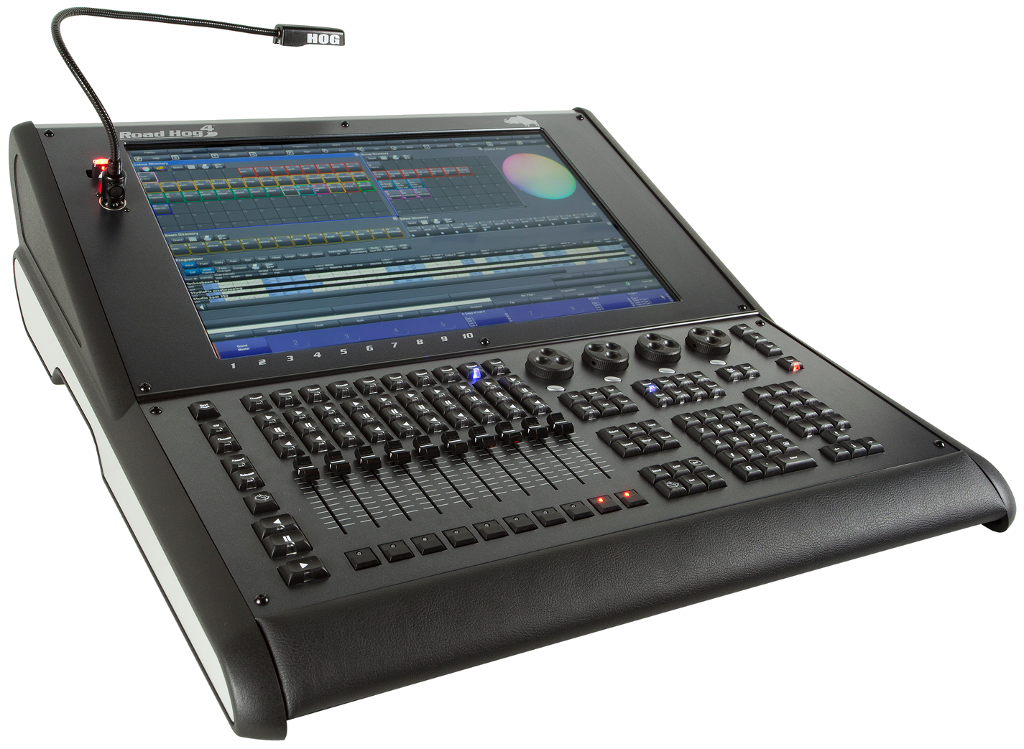
\includegraphics[width=10cm,scale=1]{resources/1_5-consolaHOG.png}
	\caption{Consola Hog4, de High End Systems. Fuente: \href{https://www.highend.com/products/consoles}{LINK a la imágen}}
	\label{fig:\thefigure}
\end{figure}

 

\section{DMX}
\subsection{definición e historia}
DMX, de \textit{Digital MultipleX}, es un estándar de comunicación digital ámpliamente utilizado para el control de sistemas de iluminación. 

El estándar DMX512, donde 512 significa que se envían 512 piezas de información, fue creado por la \textit{United States Institute for Theatre Technology} (USITT) en 1986 y transformado en DMX512/1990 tras una revisión de la USITT. En 1998 la \textit{Entertainment Services and Technology Association} (ESTA) cuadró DMX dentro de los estándares ANSI, modificación que fue aprovada por el instituto (ANSI) en 2004. Finalmente, en 2008 DMX tuvo una nueva revisión y se llegó a la versión actual llamada "E1.11 – 2008, USITT DMX512-A", o simplemente DMX512-A. A pesar de esto, el nombre comúnmente conocido del estándar es simplemente DMX, aunque no es indistinto ya que hay diferencia de compatibilidad entre las diferentes versiones.


\subsection{Capa física}
\subsubsection{Cableado y conectores}
DMX empléa el estándar EIA-485 como capa física, por lo que emplea por lo menos 3 lineas; A, B y C, en donde A y B es por los datos son transmidos, y C es masa. Los conectores utilizados son los XLR, tanto de 5 como de 3 pines. Un ejemplo del cable se puede ver en la figura \ref{fig:1.6} \\

\begin{figure}[!ht]
	\centering
	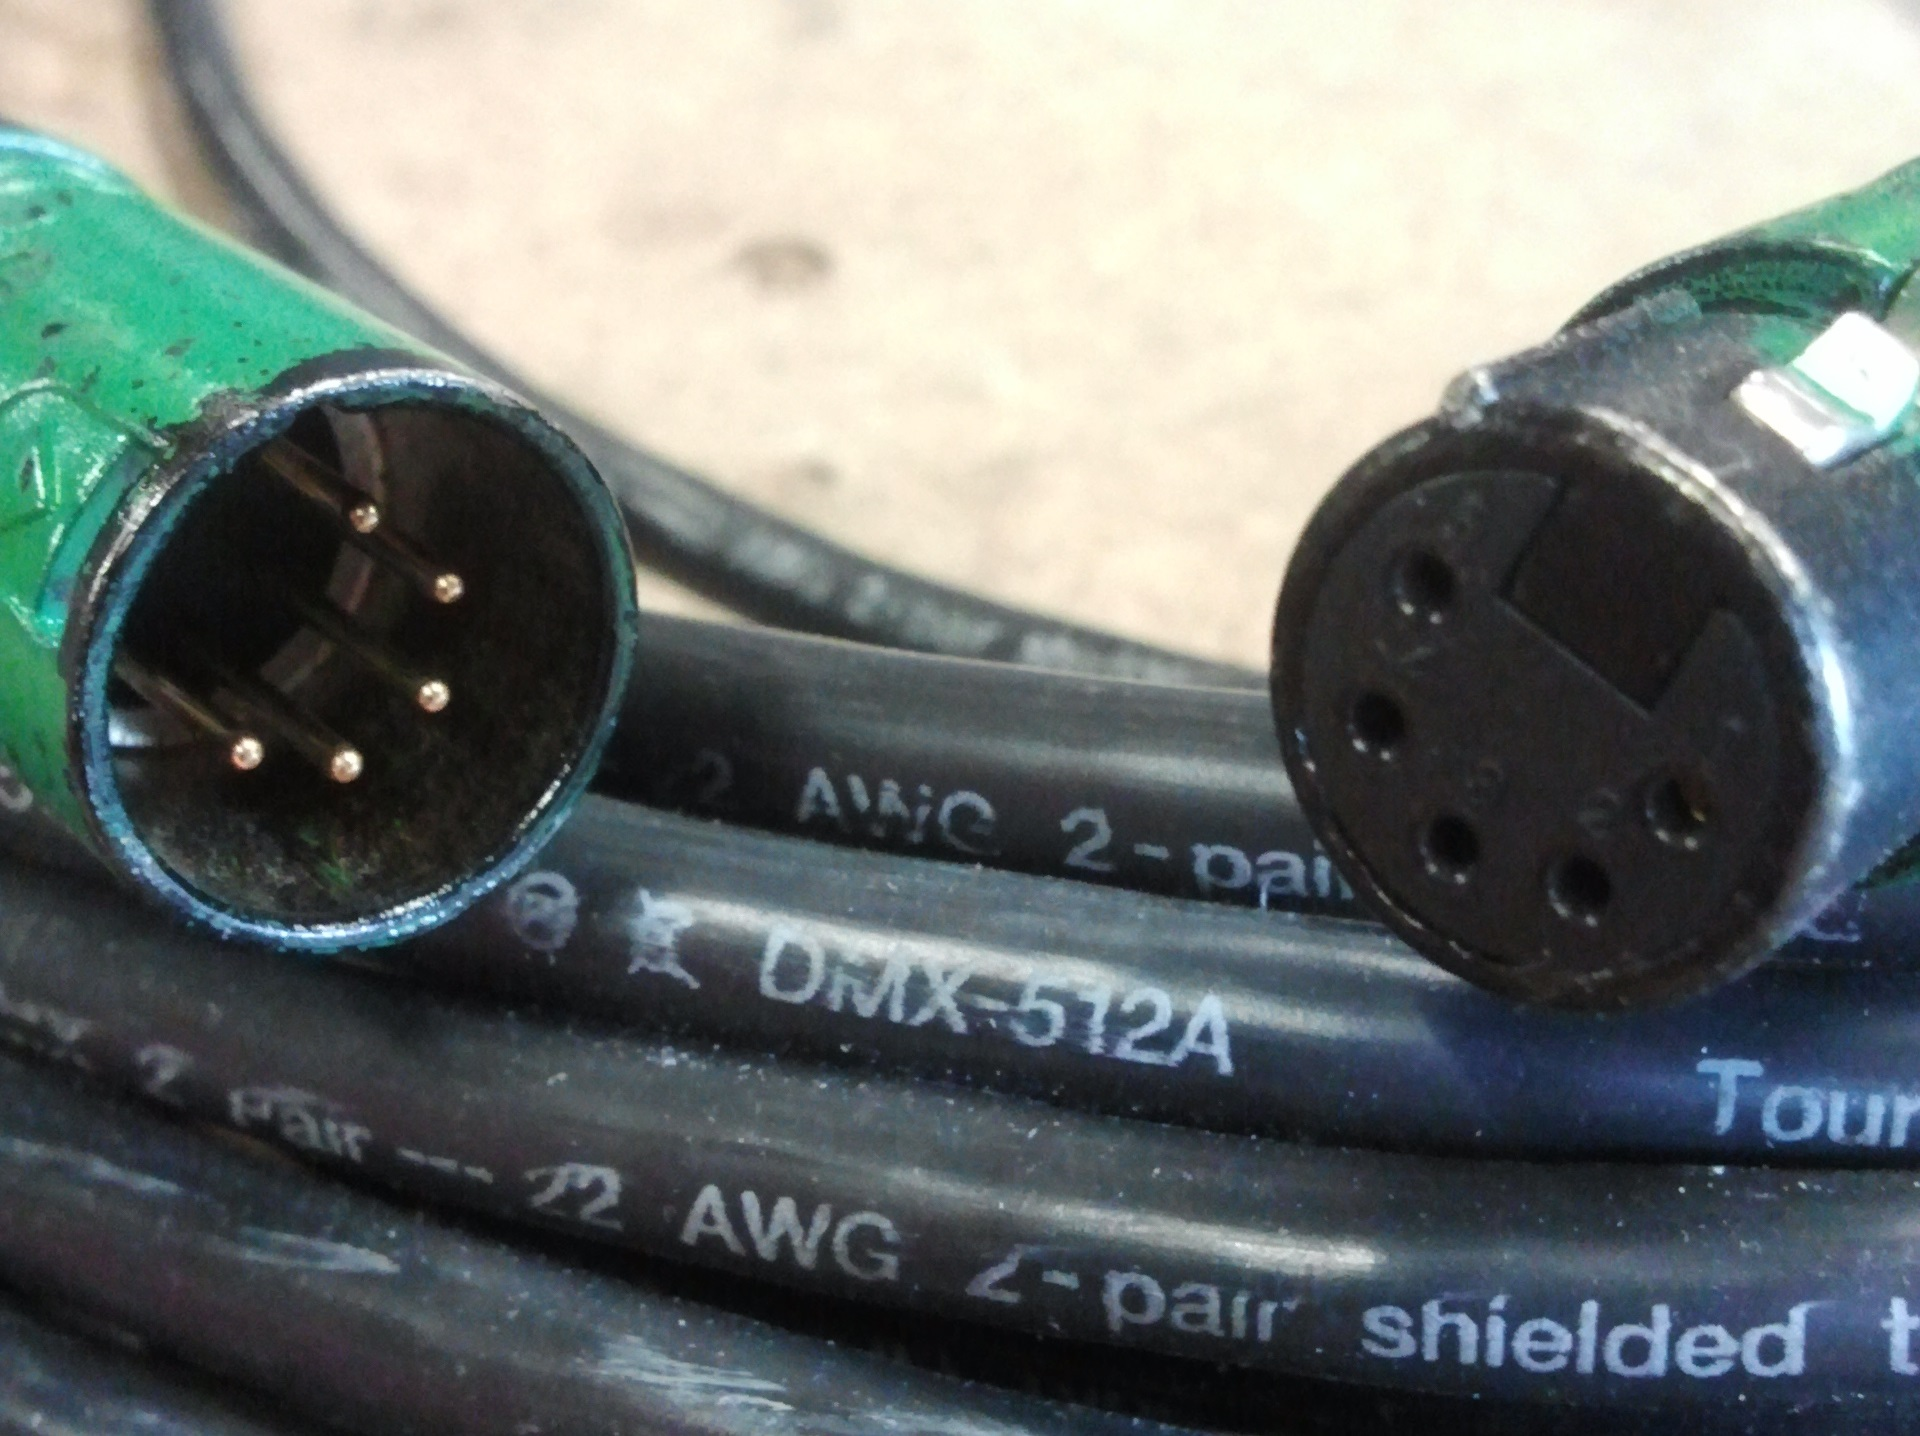
\includegraphics[width=8cm,scale=1]{resources/1_6-cableDMX.jpg}
	\caption{Cable DMX con conector XLR5. Fuente: wikipedia}
	\label{fig:\thefigure}
\end{figure}

\subsubsection{Topología}
La red de DMX consiste en un maestro y varios esclavos, conectados con una topología de bus multidrop (MDB) con nodos conectados entre sí, lo que normalmente se denomina como topología \textit{daisy chain}. En otras palabras, todos los equipos a controlar tienen una entrada y una salida conectadas entre sí, de manera tal de que se puede conectar un equipo y apartir de este equipo conectar el siguiente, y así sucesivente, como se ve en la figura \ref{fig:1.7}. Esto permite que el conexionado sea simple y que la red pueda ser fácilmente extendida.

\begin{figure}[!ht]
	\centering
	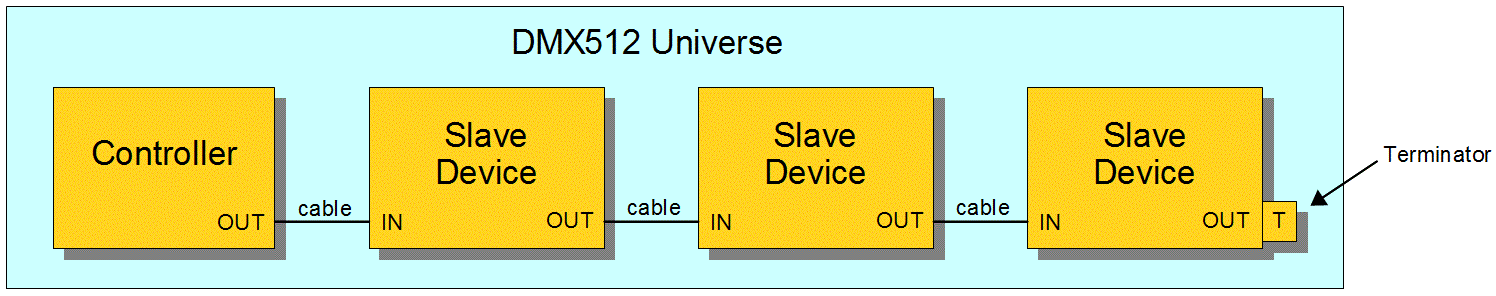
\includegraphics[width=15cm,scale=1]{resources/1_7-topologiaDMX.png}
	\caption{Conexionado en una red DMX. Fuente: wikipedia}
	\label{fig:\thefigure}
\end{figure}

\subsubsection{Señal}
Al emplear el estándar EIA-485 la señal es de tipo diferencial, de una frecuencia de 250KHz.


\subsection{Capa de enlace de datos}
\textcolor{FIXME}{canales, addressamiento, forma de paquete paquetes, direccionalidad (uni)}\\
y paquetes de largo variable para la comunicación entre maestro y esclavo (que suele ser unidireccional).

\subsection{RDM}




\section{Updown}
\subsection{Definición}

\subsection{Blackout}
Black-out es una empresa productora y proveedora de tecnología, cuyo objetivo es generar contenido audiovisual para grandes eventos. Para cumplir con este objetivo la empresa dedica recursos al desarrollo de productos tecnológicos innovadores, como es el caso de los equipos destinados a generar las llamadas Esculturas cinéticas (Kinetic sculpture en inglés).\\

\subsection{Productos que compiten en el mercado}
El equipos más conocido empleado para estas aplicaciones es el \href{http://www.eastsunlite.com/p31.html}{OrbisFly}, de \href{https://www.kinetic-lights.com/}{Kinetic Lights}. Estos dispositivos de orígen Chino trabajan con una esfera RGB de peso estándar de 1Kg, aunque soporta un peso máximo de 2Kg, que puede descender hasta 9 metros. Dispone de un display LCD y botoneras para el testeo y configuración el equipo\\

\newpage
\section{Justificación del proyecto}
La empresa Black-out se encargó de comenzar el desarrollo de los Up-down; los equipos necesarios para crear los efectos de esculturas cinéticas. El inconveniente es que solo fue armada la parte mecánica del mismo, ya que a efectos prácticos el firmware que se utilizaba para manejar el conjunto era pobre.\\
Ante la necesidad que se tiene que el equipo controle la posición y velocidad de la carga, y que además verifique errores de hardware durante su uso para evitar accidentes, surgió la necesidad de buscar a alguien capacitado para mejorar la programación y terminar el proyecto.
Es entonces que se presentó la oportunidad de realizar un trabajo en la empresa con el objetivo de completar lo que falta del proyecto, hacer que este cumpla ciertas especificaciones técnicas, y crear documentación sobre el firmware y software de prueba de hardware para que más equipos de las mismas características puedan ser producidos. De esta manera, para completar el objetivo se debe:
\begin{itemize}
	\item Implementar un control automático de posición y velocidad de la carga movida por el equipo para lograr los efectos deseados.
	\item Permitir el cambio de los setpoints de posición y velocidad mediante comandos DMX enviados al equipo por una consola de luces, como puede ser una \href{https://www2.highend.com/products/controllers/Hog4Console.asp}{consola HOG4}
	\item Manejar errores y excepciones de hardware para lograr que el producto sea seguro, siendo que será instalado en eventos con un alto nivel de concurrencia.
\end{itemize}




